\section{No rule leads across collections}\label{sec:coll}

Table~\ref{tab:collections2} and Figure~\ref{fig:collections} give the accuracy of every rule on every collection. Three observations organise the rest of the paper.

\begin{table}[t]
\caption{Accuracy (fraction of pairs oriented correctly; exact ties half) of twelve rules on seven collections. ``--'': not run, or no value returned for most pairs (TRA on the Bernoulli, changepoint and Malus collections). The Bernoulli, changepoint and Malus collections have $8$, $7$ and $4$ distinct edges; intervals that account for clusters are in Appendix Table~\ref{tab:collections_ci}.}
\label{tab:collections2}
\small
\setlength{\tabcolsep}{4pt}
\begin{tabular}{@{}lccccccc@{}}
\toprule
Rule & T\"ub. & iid & walks & Sachs & Bern. & Chgpt. & Malus\\
 & (102) & (94) & (122) & (17) & (16) & (70) & (48)\\
\midrule
IGCI & 0.56 & 0.94 & 0.89 & 0.65 & 0.00 & 0.00 & 0.96\\
RECI & 0.61 & 0.98 & 0.94 & 0.53 & 0.25 & 1.00 & 0.56\\
ANM-HSIC & 0.61 & 0.72 & 0.63 & 0.59 & 0.31 & 0.47 & 0.33\\
Pairwise LiNGAM & 0.61 & 0.78 & 0.71 & 0.53 & 0.88 & 0.43 & 0.40\\
PDM & 0.40 & 0.93 & 0.84 & -- & -- & -- & --\\
LOCI & 0.65 & 0.77 & 0.68 & 0.47 & -- & -- & --\\
ANM, Gaussian process & 0.55 & 0.77 & 0.67 & 0.56 & -- & -- & --\\
Compression, first impl. & 0.61 & 0.30 & 0.61 & 0.76 & -- & -- & --\\
Compression, faithful & 0.67 & 0.38 & 0.52 & 0.65 & 0.50 & 1.00 & 0.60\\
TRA & 0.65 & 0.86 & 0.61 & 0.59 & -- & -- & --\\
AVICI & 0.59 & 0.90 & 0.56 & 0.53 & 0.62 & 0.40 & 0.02\\
RESIT & 0.61 & 0.71 & 0.65 & 0.47 & 0.31 & 0.50 & 0.50\\
\bottomrule
\end{tabular}
\end{table}

\begin{figure}[t]
\centering
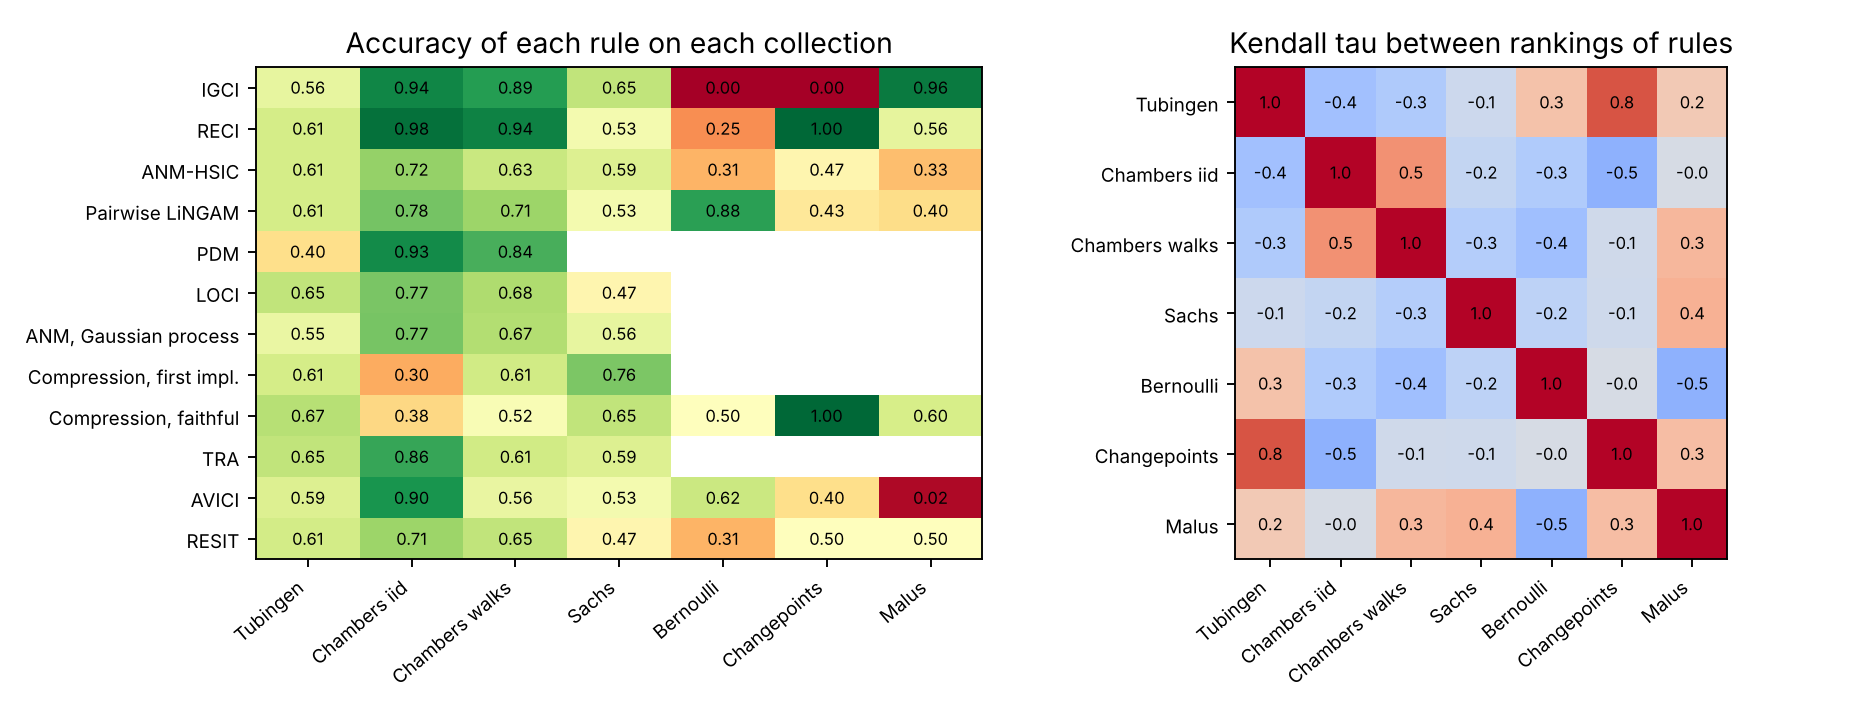
\includegraphics[width=\linewidth]{figs/collections.png}
\caption{Left: accuracy of each rule on each collection. Right: Kendall rank correlation between the orderings of the rules on two collections (rules run on both; at least five).}
\label{fig:collections}
\end{figure}

\paragraph{(1) The leader changes with the collection.} The best rule is faithful compression on T\"ubingen ($66.7\%$; LOCI and TRA at $64.7$ and $64.6\%$), RECI on both chamber collections with independent or random-walk actuators ($97.9\%$ and $94.3\%$), our first compression implementation on the 17 Sachs pairs ($76.5\%$; the faithful one $64.7\%$), pairwise LiNGAM on the Bernoulli collection ($87.5\%$), RECI and the faithful compression together on the changepoint collection ($100\%$ for both), and IGCI on the Malus collection ($95.8\%$). No rule is above $70\%$ on more than three collections, and five of the twelve rules lead at least one collection (counting the two compression implementations separately; our first implementation leads Sachs by $13$ against $11$ of $17$ pairs for the faithful one, and the faithful one was chosen to match a published figure, so its leads on T\"ubingen and the changepoints partly reflect that choice).

\paragraph{(2) Rules that agree on one collection can disagree on the next.} In our implementation IGCI is the second-best rule on both chamber collections ($93.6$ and $88.5\%$) and the best on Malus, yet it orients every one of the $16$ Bernoulli pairs and every one of the $70$ changepoint pairs the wrong way ($0\%$): the cause has many ties (a grid of $101$ levels with about $20$ rows per level in the Bernoulli collection, four piecewise-constant levels in each changepoint experiment), and we conjecture, without having diagnosed it, that the entropy estimator is then degenerate after the small jitter that breaks the ties, so that the decision is the same for every pair. RECI, best or tied-best on three collections, is at $25\%$ on the Bernoulli pairs. The pretrained AVICI model, run on two-variable inputs, is at $90.4\%$ on the i.i.d.\ chambers and at $2.1\%$ on Malus, where it prefers the reverse direction for $47$ of the $48$ pairs. Compression is at $100\%$ on the changepoint pairs and at $38.3\%$ on the i.i.d.\ chambers.

\paragraph{(3) Rankings of rules do not clearly transfer.} The Kendall correlation between the ordering of the rules on T\"ubingen and on the i.i.d.\ chambers is $-0.38$ and against the walk pairs $-0.30$; the two chamber collections agree with each other ($+0.53$); T\"ubingen against Sachs is $-0.12$. These are negative or near zero, but with a permutation test over the rules none is distinguishable from zero ($p=0.11$, $0.21$, $0.67$): the T\"ubingen accuracies span about twelve points with intervals of $\pm0.10$, and the ordering of the rules on that collection is mostly noise. Other pairs of collections give positive values (T\"ubingen against changepoints $+0.79$, $p=0.02$, seven rules; against Bernoulli $+0.26$ and Malus $+0.21$). The full matrix with permutation $p$-values is in Appendix Table~\ref{tab:kendall}. What the matrix does not show is a shared ranking: a rule that leads T\"ubingen says little, in either direction, about a collection from a device with a documented graph. The two compression variants and PDM are counted as rules, and the i.i.d.\ and walk collections come from the same devices.

\paragraph{Cautions.} The Bernoulli, changepoint and Malus collections consist of $8$, $7$ and $4$ distinct edges, repeated across seeds or experiments, with the same cause variable (\texttt{load\_in}, or the two polarisers); they are small, correlated sets of regimes, not samples of mechanisms, and we use them as such. Sachs has $17$ pairs. The T\"ubingen collection mixes pairs from several fields and its weights downweight groups of similar pairs; unweighted accuracy is used here unless stated.
